\documentclass[conference,a4paper]{IEEEtran}

% Escritura mejorada de fórmulas matemáticas
\usepackage{amsmath}

% Inserción de gráficos
\usepackage{graphicx}

% Escritura de pseudocódigo
\usepackage[kw]{pseudo}

% Escritura mejorada de tablas
\usepackage{booktabs}

% Escritura mejorada de citas bibliográficas
\usepackage{cite}

\usepackage{pgfplots}
\pgfplotsset{compat=1.18}
\usepackage{tikz}
\usepackage{caption}




% Macros traducidas
\def\contentsname{Índice general}
\def\listfigurename{Índice de figuras}
\def\listtablename{Índice de tablas}
\def\refname{Referencias}
\def\indexname{Índice alfabético}
\def\figurename{Fig.}
\def\tablename{TABLA}
\def\partname{Parte}
\def\appendixname{Apéndice}
\def\abstractname{Resumen}
% IEEE specific names
\def\IEEEkeywordsname{Palabras clave}
\def\IEEEproofname{Demostración}


\begin{document}

\title{Aprendizaje de un agente de Otelo mediante self-play y Monte Carlo Tree Search}

\author{
  \IEEEauthorblockN{Javier Carrasco Águilar}
  \IEEEauthorblockA{
    \textit{Dpto. Ciencias de la Computación e Inteligencia Artificial}\\
    \textit{Universidad de Sevilla}\\
    Sevilla, España\\
    javcaragu1@alum.us.es}
  
  \and
  
  \IEEEauthorblockN{Alejandro Silvestre García}
  \IEEEauthorblockA{
    \textit{Dpto. Ciencias de la Computación e Inteligencia Artificial}\\
    \textit{Universidad de Sevilla}\\
    Sevilla, España\\
    alesilgar2@alum.us.es}
}

\maketitle


% Resumen
\begin{abstract}
  En este trabajo se llevará a cabo el desarrollo de un agente inteligente para jugar al juego de Otelo. La finalidad es que se pueda jugar contra la máquina como si fuera un jugador real. El agente será basado en Monte Carlo Tree Search (MCTS) con el enfoque de UpperConfidenceBoundTree(UCT) \cite{b4}.

  Se realizaron varios experimentos para analizar la influencia de los criterios de selección del algoritmo UCT y de los principales parámetros de entrenamiento de la red neuronal. Los resultados muestran que el uso de una red neuronal como función de evaluación mejora la eficiencia del proceso de búsqueda y que los criterios \textit{max-robust} y \textit{secure} obtienen, en general, los mejores resultados. Asimismo, se observó que se necesitan al menos 30 épocas para tener unos datos de precisión y pérdida más estables y significativos, mientras que incrementar el número no merece la pena pues la diferencia resultados es muy marginal. En conclusión, el trabajo demuestra la viabilidad de combinar UCT y redes neuronales para construir un agente inteligente de Otelo capaz de aprender mediante self-play.
  
\end{abstract}


% Palabras claves
\begin{IEEEkeywords}
  Inteligencia Artificial, Otelo, UCT, red neuronal, épocas
\end{IEEEkeywords}


\section{Introducción}

Históricamente, los juegos de tablero han sido muy útiles para entrenar modelos de Inteligencia Artificial. Desde el primer algoritmo desarrollado por Alan Turing en 1948 para jugar al ajedrez \cite{b1}, las mecánicas de estos juegos se pueden usar para entrenar agentes capaces de tomar decisiones estratégicas que permiten desarrollar algoritmos que pueden aplicarse a otros dominios distintos. 

En nuestro caso, usando el juego Otelo, implementaremos un agente basado en Monte Carlo Tree Search (MCTS) con el enfoque de Upper Confidence Bound Tree(UCT). Se utilizará una red neuronal para estimar el valor de las posiciones, guiando así la expansión y selección de nodos dentro del árbol de búsqueda. No se hará uso de una heurística explícita.

El juego se ha implementado a través de una matriz con 8 filas y 8 columnas y funciones para gestionar las reglas del juego. Se incluyen procedimientos para generar el tablero inicial, calcular los movimientos legales, aplicar jugadas volteando las fichas correspondientes y calcular la puntuación de cada jugador. Además, incluye una interfaz por consola en la que se probaron las interacciones básicas y el correcto funcionamiento. Esta implementación sirve como base sobre la que se integran posteriormente los algoritmos de búsqueda y aprendizaje utilizados en el proyecto.

El algoritmo está sacado del artículo \cite{b2}, donde se describe un pseudocódigo del algoritmo UCT, del que haremos una implementación propia para el juego de Otelo. También crearemos una red neuronal entrenada para utilizarla en la función DefaultPolicy(s), que forma parte del algoritmo. La función de la red es sustituir los rollouts aleatorios por predicciones del resultado de la partida a partir del estado actual del tablero. Para este entrenamiento se generan partidas automáticas entre instancias del propio agente, etiquetando cada posición con el resultado final de la partida.

La implementación ha sido realizada con Python. Además, se ha desarrollado una interfaz gráfica con PyGame para poder jugar contra el agente.

El resto del documento se organiza como sigue. La sección~\ref{sec:Preliminares} introduce los fundamentos teóricos del algoritmo UCT y de las redes neuronales empleadas, así como trabajos relacionados. La sección~\ref{sec:Metodologia} describe en detalle la implementación desarrollada. La sección~\ref{sec:Resultados} presenta los experimentos realizados y los resultados obtenidos. La sección~\ref{sec:Uso de IA} explica el uso de inteligencia artificial generativa en el proyecto. Finalmente, la sección~\ref{sec:Conclusiones} recoge las conclusiones y posibles líneas de trabajo futuro. 

\section{Preliminares}\label{sec:Preliminares}

En este proyecto se ha empleado un proceso de self‑play, donde la propia IA genera sus datos jugando partidas contra sí misma. Para decidir los movimientos durante estas partidas se utiliza el algoritmo UCT (Upper Confidence bounds applied to Trees), una variante de Monte Carlo Tree Search que permite seleccionar movimientos de manera mas eficiente, ayudando a un aprendizaje más rápido. Cada partida se etiqueta según el resultado final (derrota, empate o victoria), lo que permitirá entrenar la red mediante aprendizaje supervisado. De esta forma, en cada iteración el modelo mejora con los datos producidos por versiones anteriores.



\subsection{\textbf{Métodos empleados}}

En este proyecto se han aplicado diversas técnicas de Inteligencia Artificial y Aprendizaje Automático para desarrollar una IA capaz de aprender a jugar a Otelo. Entre los métodos utilizados destacan los siguientes:

\begin{itemize}
    \item \textbf{Búsqueda en el espacio de estados mediante Monte Carlo Tree Search con UCT}: se emplea la variante UCT para equilibrar exploración y explotación durante la selección de movimientos, construyendo un árbol de búsqueda basado en simulaciones y estadísticas de visitas y recompensas.
    
    \item \textbf{Evaluación de nodos mediante simulaciones y red neuronal}: los estados del juego se evalúan mediante la predicción de una red neuronal que estima la probabilidad de victoria, acelerando la búsqueda y mejorando la calidad de las decisiones.
    
    \item \textbf{Self-play para la generación automática de datos}: la IA juega partidas contra sí misma, utilizando MCTS (versión UCT) para seleccionar movimientos. Esto permite generar grandes cantidades de datos en un breve periodo de tiempo.
    
    \item \textbf{Entrenamiento iterativo}: el modelo se mejora de forma iterativa, utilizando en cada iteración los datos generados por versiones anteriores de la propia IA, lo que permite un proceso de mejora continua.
    
    \item \textbf{Aprendizaje supervisado}: las posiciones generadas se etiquetan según el resultado final de la partida (victoria, empate o derrota), y se utiliza una red neuronal multicapa (MLP) para aprender a clasificar el valor de cada estado del tablero.
    
    \item \textbf{Técnicas de clasificación}: se emplean funciones de pérdida de clasificación multiclase, optimización mediante Adam (Adaptative Moment Estimation) y entrenamiento por minibatches para ajustar los parámetros de la red neuronal.

    \item \textbf{Interfaz gráfica}: se ha empleado de base una interfaz gráfica de PyGame de un proyecto nuestro anterior. Naturalmente ha sufrido bastantes cambios pues era para un juego totalmente distinto. Solo se ha podido rescatar la estructura general y funciones básicas como crear la ventana del juego, el header y la asignación de teclas como 'ESC' para cerrarlo.
\end{itemize}


Por último, se debe hacer un uso correcto de las referencias bibliográficas,
para que el lector pueda acceder a más información~\cite{b2}. Todas las
referencias al final del documento deben ser citadas al menos una vez.


\subsection{\textbf{Trabajo Relacionado}}

Se tuvo en cuenta "A Survey of Monte Carlo Tree Search Method" para obtener de el la idea general y ayuda a la implementacion de UCT.

\section{Metodología}\label{sec:Metodologia}

\subsection{\textbf{Implementación del juego}}

La implementación del juego de Otelo consta de tres componentes principales: la representación del tablero, las funciones que implementan las reglas del juego y la interfaz de usuario. Esta organización ayuda a integrar posteriormente los algoritmos de búsqueda y aprendizaje.

\subsubsection{\textbf{Representación del tablero}}

El tablero se modela como una matriz de 8$\times$8, donde cada casilla contiene un valor entero que indica su estado: \texttt{0} para casilla vacía, \texttt{1} para ficha blanca y \texttt{2} para ficha negra. La función \texttt{nuevo\_tablero} inicializa el estado según la configuración del principio del juego, colocando las cuatro fichas centrales cruzadas entre si. Esta representación matricial permite recorrer el tablero de manera eficiente y aplicar los movimientos en todas las direcciones.

\subsubsection{\textbf{Funciones principales del juego}}

Las reglas de Otelo se implementan mediante un conjunto de funciones. La función \texttt{movimientos\_legales} calcula todas las jugadas válidas para un jugador dado, explorando cada dirección y comprobando si existe una secuencia de fichas del oponente seguida de una ficha del jugador. La función \texttt{aplicar\_movimiento} coloca la ficha del jugador en la casilla seleccionada y voltea todas las fichas entre esta última y la correspondiente. Otras funciones auxiliares, como \texttt{cuenta\_fichas} o \texttt{parsea\_entrada}, permiten gestionar la puntuación y convertir la entrada del usuario en coordenadas del tablero.

\subsubsection{\textbf{Interfaz de usuario}}

La función \texttt{jugar\_cli} proporciona una interfaz de línea de comandos que permite jugar partidas completas. En cada turno se muestra el tablero, se indican los movimientos legales y se solicita al usuario que introduzca su jugada. La interfaz gestiona también los casos en los que un jugador debe pasar, y determina el resultado final de la partida una vez que ambos jugadores no pueden realizar más jugadas. Esta interfaz sirve como entorno de prueba para validar la lógica del juego y como base para integrar posteriormente agentes automáticos.
Además, incluye una interfaz gráfica que emplea la librería PyGame que permite el juego contra la IA seleccionando quién empieza el juego (eligiendo el color) para que el usuario pueda jugar de manera más cómoda. 


\subsection{\textbf{Algoritmo UCT}}

La implementación del agente se estructura en torno al algoritmo UCT,
que está implementado en el fichero \texttt{algoritmo\_uct.py}.Dicho fichero se divide en tres componentes (clases) principales que serán descritos a continuación.

\subsubsection{\textbf{Representación del estado}}

La clase \texttt{EstadoOthello} encapsula el estado del juego y envuelve el tablero de juego (una matriz $8 \times 8$ de enteros) junto con el turno del jugador activo. Esta clase tiene los métodos necesarios para clonar el estado, obtener los movimientos válidos, aplicar un movimiento y determinar si la partida ha terminado y quién ha ganado. Internamente, la representación usa los valores $0$
(casilla vacía), $1$ (ficha blanca) y $2$ (ficha negra).

\subsubsection{\textbf{Estructura del árbol: clase Nodo}}

Cada nodo del árbol MCTS se representa mediante la clase \texttt{Nodo}, que
almacena los siguientes atributos:

\begin{itemize}
  \item \texttt{estado}: copia del estado del juego en ese nodo.
  \item \texttt{jugador}: jugador que acaba de mover para llegar a este nodo.
  \item \texttt{movimiento}: jugada que generó este nodo desde su padre,
  representada como una tupla $(\text{fila}, \text{columna})$.
  \item \texttt{padre}: nodo padre en el árbol, o \texttt{None} en el caso de ser la raíz.
  \item \texttt{hijos}: lista de nodos hijo ya expandidos desde este nodo.
  \item \texttt{n\_visitas}: número de veces que el nodo ha sido visitado.
  \item \texttt{n\_victorias}: valor acumulado de recompensas recibidas.
  \item \texttt{movs\_sin\_expandir}: lista de movimientos aún no explorados,
  barajada aleatoriamente en la construcción del nodo.
\end{itemize}


\subsubsection{\textbf{Implementación del pseudocódigo del Algoritmo UCT}}

El agente se implementa en la clase \texttt{AgenteUCT}, que ejecuta un número configurable de iteraciones por jugada. Cada iteración aplica las cuatro fases del algoritmo UCT descritas en pseudocódigo en \cite{b2}:

\begin{enumerate}
  \item \textbf{Tree Policy}: se desciende por el árbol
  eligiendo en cada nivel el hijo con mayor valor UCB1, definido como:
  \begin{equation}
    \text{UCB1} = \frac{v_i}{n_i} + c \sqrt{\frac{\ln N}{n_i}}
    \label{eq:ucb1}
  \end{equation}
  donde $v_i$ es el valor acumulado del hijo $i$, $n_i$ sus visitas, $N$ las
  visitas del nodo padre y $c = \sqrt{2}$ la constante de exploración. El
  descenso se detiene al encontrar un nodo no completamente expandido o terminal.

  \item \textbf{Expand}: si el nodo no está completamente expandido, se toma
  un movimiento aún no explorado, se aplica sobre una copia del estado y se
  añade un nuevo nodo hijo al árbol.

  \item \textbf{Default Policy}: se estima la recompensa desde el nodo expandido. Si se dispone de una red neuronal entrenada, se usa su predicción directamente, evitando la simulación completa. En caso contrario, se realiza un rollout aleatorio hasta el final de la partida. En ambos casos el valor devuelto pertenece al intervalo $[-1, 1]$, donde $+1$ representa victoria y $-1$ derrota para el jugador activo.

  \item \textbf{Backup}: la recompensa obtenida se
  propaga hacia arriba por el árbol hasta la raíz, sumándose en los nodos del jugador activo y restándose en los del oponente, actualizando en cada nodo los contadores \texttt{n\_visitas} y \texttt{n\_victorias}.
  
\end{enumerate}

Una vez completadas todas las iteraciones, el agente selecciona como jugada
final el hijo de la raíz según uno de los criterios descritos en \cite{b2}.
En este trabajo se han evaluado tres de ellos:

\begin{itemize}
  \item \textit{Max child}: selecciona el hijo con mayor valor medio
  ($n\_victorias / n\_visitas$). Es el criterio más directo, pero sensible a fluctuaciones
  estadísticas en nodos poco visitados.
  \item \textit{Robust child}: selecciona el hijo con mayor número de visitas.
  Es más estable que \textit{max child}, ya que el nodo más visitado refleja
  una ventaja consistente a lo largo de todo el proceso de búsqueda, sin verse afectado por valores medios inflados por azar.
  \item \textit{Max-robust child}: combina los dos criterios anteriores,
  seleccionando el hijo que simultáneamente tenga el mayor número de visitas
  y el mayor valor medio. Si ningún hijo cumple ambas condiciones a la vez,
  el proceso de búsqueda continúa hasta que alguno las satisfaga \cite{b2}.
  \item \textit{Secure child}: selecciona el hijo que maximiza una cota inferior
  de confianza, definida como:
  \begin{equation}
    \frac{v_i}{n_i} - c\sqrt{\frac{\ln N}{n_i}}
    \label{eq:secure}
  \end{equation}
  Este criterio prima la seguridad frente a la ambición: elige el hijo cuyo
  rendimiento mínimo estimado es mayor, penalizando los nodos con pocas visitas
  aunque tengan un valor medio alto.

  A continuación se muestra el pseudocódigo de la función desarrollada para elegir los criterios.

  \begin{figure}
\begin{pseudo}*
  \hd{\fn{MejorHijoFinal}}(\text{nodo}, \text{criterio}) \\*
  \multicolumn{2}{l}{\textbf{Entrada}: un nodo del árbol MCTS y un criterio de selección} \\*
  \multicolumn{2}{l}{\textbf{Salida}: el hijo de \text{nodo} seleccionado según el criterio} \\
  if \( \text{criterio} = \textit{"max"} \) entonces \\+
    devolver \( \arg\max_{h \in \text{hijos}} \dfrac{n\_victorias}{n\_visitas} \) \\-
  elif \( \text{criterio} = \textit{"robust"} \) entonces \\+
    devolver \( \arg\max_{h \in \text{hijos}} \; n\_visitas \) \\-
  elif \( \text{criterio} = \textit{"max-robust"} \) entonces \\+
    \( vis^* \leftarrow \max_{h} \; n\_visitas \) \\
    \( vic^* \leftarrow \max_{h} \; n\_victorias / n\_visitas \) \\
    \( C \leftarrow \{ h \in \text{hijos} \mid n\_visitas = vis^* \wedge n\_victorias / n\_visitas = v^* \} \) \\
    if \( C \neq \emptyset \) entonces \\+
      devolver cualquier \( h \in C \) \\-
    si no entonces \\+
      devolver \( \arg\max_{h \in \text{hijos}} \; n\_visitas \) \\-\\-
  elif \( \text{criterio} = \textit{"secure"} \) entonces \\+
    devolver \( \displaystyle\arg\max_{h \in \text{hijos}}
      \left( \frac{n\_victorias}{n\_visitas} - c\sqrt{\frac{\ln N}{n\_visitas}} \right) \)
\end{pseudo}
\caption{Función \texttt{MejorHijoFinal}: selección del movimiento final}
\label{pcd:mejorHijoFinal}
\end{figure}
\end{itemize}

En la sección~\ref{sec:Resultados} se compara el rendimiento de los tres
criterios en términos de accuracy y loss del modelo entrenado con cada uno
de ellos.
Una vez que están todas las iteraciones, el agente selecciona como jugada 
final el hijo de la raíz con mayor número de visitas, que es el criterio denominado como \textit{robust child} en \cite{b2}. Este criterio es más estable que elegir el hijo con mayor valor medio (\textit{max child}), ya que un nodo poco visitado puede llegar tener un valor medio alto por azar, mientras que el más visitado refleja una ventaja consistente a lo largo de todo el proceso de búsqueda.

\subsection{Red neuronal}

La red neuronal utilizada en este proyecto actúa como una función de evaluación aproximada del estado del tablero

\vspace{5em}






\subsubsection{Representación de las entradas}

\begin{center}
\begin{minipage}{0.95\linewidth}
\small
\begin{pseudo}*
  \hd{\fn{CodificarTablero}}(\text{tablero}, \text{jugador}) \\*
  \multicolumn{2}{l}{\textbf{Entrada}: matriz 8$\times$8 con valores \{0,1,2\}} \\
 \textbf{Salida}: vector de 64 características \\
  \( v \leftarrow [] \) \\
  por cada casilla \( c \) en el tablero\\+
    si \( c = \text{jugador} \) entonces \\+
      añadir \( +1 \) a \( v \) \\-
    si \( c = \text{oponente} \) entonces \\+
      añadir \( -1 \) a \( v \) \\-
    si \( c = 0 \) entonces \\+
      añadir \( 0 \) a \( v \) \\-\\-
  devolver \( v \)
\end{pseudo}
\captionof{figure}{Codificación del tablero como vector de entrada}
\label{pcd:codificarTablero}
\end{minipage}
\end{center}



\subsubsection{Arquitectura del modelo}

\begin{center}
\begin{minipage}{0.95\linewidth}
\small
\begin{pseudo}*
  \hd{\fn{ConstruirRed}}() \\*
  \multicolumn{2}{l}{\textbf{Salida}: modelo MLP compilado} \\
  crear modelo secuencial \\
  añadir capa densa de tamaño \(h_1\) con activación ReLU \\
  añadir capa densa de tamaño \(h_2\) con activación ReLU \\
  añadir capa de salida de tamaño 3 con activación Softmax \\
  compilar modelo con: \\+
    pérdida = \textit{Sparse Categorical Crossentropy} \\
    optimizador = Adam \\
    métrica = accuracy \\-
  devolver modelo
\end{pseudo}
\captionof{figure}{Arquitectura de la red neuronal}
\label{pcd:arquitecturaRed}
\end{minipage}
\end{center}

\subsubsection{Entrenamiento supervisado}

\begin{center}
\begin{minipage}{0.95\linewidth}
\small
\begin{pseudo}*
  \hd{\fn{EntrenarRed}}(\text{modelo}, X, y, \text{epochs}, \text{batch}) \\*
  \multicolumn{2}{l}{\textbf{Entrada}: datos, etiquetas y parámetros de entrenamiento} \\
  \textbf{Salida}: modelo entrenado \\
  para \( e = 1 \) hasta \text{epochs} hacer \\+
    dividir \( X \) en minibatches de tamaño \text{batch} \\
    para cada minibatch \( (X_b, y_b) \) hacer \\+
      modelo.\texttt{train\_step}($X_b, y_b$) \\-
    actualizar métricas de entrenamiento \\-
  devolver modelo
\end{pseudo}
\captionof{figure}{Proceso de entrenamiento supervisado}
\label{pcd:entrenamientoRed}
\end{minipage}
\end{center}




\subsection{Integración de la red neuronal}

La red neuronal se integra en la fase de simulación. En lugar de simular la
partida hasta el final, se codifica el tablero actual como un vector de $64$
valores desde la perspectiva del jugador activo ($+1$ ficha propia, $-1$ ficha
del oponente, $0$ casilla vacía) y se pasa a la red, que devuelve tres
probabilidades correspondientes a derrota, empate y victoria. El valor usado
como recompensa es $P(\text{victoria}) - P(\text{derrota})$, que produce un
escalar en $[-1, 1]$ coherente con el esquema de retropropagación del algoritmo.

\section{Resultados}\label{sec:Resultados}
A continuación vamos a explicar los distintos experimentos realizados y los resultados obtenidos al probar distintas formas de entrenar modelos.

\subsection{Criterios de selección y épocas}

El primer experimento realizado ha sido comprobar los resultados de \textbf{Accuracy} y \textbf{Loss} al entrenar el modelo con partidas generadas por cada uno de los cuatro criterios de selección (\textit{max, max-robust, robust, secure}). Se hicieron con los siguientes parámetros: \textbf{\textit{50 partidas}}, \textbf{\textit{10 épocas}}, \textbf{\textit{128 batch-size}}, \textbf{\textit{0.01 learning rate}}. A continuación se presentará una tabla con los resultados.

\begin{table}[h]
\centering
\caption{Resultados del entrenamiento según criterio de selección final}
\label{tab:criterios}
\begin{tabular}{lcc}
\hline
\textbf{Criterio} & \textbf{Accuracy} & \textbf{Loss} \\
\hline
max-robust & 0.9655 & 0.0897 \\
robust     & 0.9650 & 0.1019 \\
max        & 0.9624 & 0.0938 \\
secure     & 0.9543 & 0.0987 \\
\hline
\end{tabular}
\end{table}

Como se puede ver en la tabla~\ref{tab:criterios}, la precisión en todos los casos es superior al 95\% por lo que nuestra red tiene una fiabilidad alta. No obstante, vemos que el criterio de selección \textit{max-robust} ha dado los mejores resultados, con el mayor \textit{Accuracy} y el menor \textit{Loss}. Aunque la precisión de \textbf{robust} es muy similar esta si tiene una perdida superior luego tiene menos fiabilidad. El resto de criterios presenta unos resultados aceptables a pesar de no ser los más destacados. Este número de épocas es muy pequeño por lo que vamos a incrementarlo para ver como se gana más precisión y disminuye la pérdida.

A continuación se ha hecho un entreno adicional de 30 épocas para \textit{max-robust} para ver la diferencia respecto a las 10 del entrenamiento anterior. (Tabla~\ref{tab:maxrobust_comparacion})

\begin{table}[h]
\centering
\caption{Comparación del rendimiento del criterio max-robust según entre las épocas 10 y 30}
\label{tab:maxrobust_comparacion}
\begin{tabular}{lcc}
\hline
\textbf{Épocas} & \textbf{Accuracy} & \textbf{Loss} \\
\hline
10 & 0.9655 & 0.0897 \\
30 & 0.9749 & 0.0451 \\
\hline
$\Delta$ (30-10) & +0.0094 & -0.0446 \\
\hline
\end{tabular}
\end{table}

Mientras que la precisión es un poco mejor, el mayor cambio es en la diferencia de la pérdida, que es de aproximadamente el 50\% respecto a las 10 épocas. Esto nos indica que la confianza y la fiabilidad mejora bastante a medida que usamos más épocas.

En el siguiente experimento que hemos hecho sobre los criterios hemos vuelto a hacer un entreno de 30 épocas pero esta vez para el criterio \textit{secure}, que era el que menor resultado dio. (Tabla~\ref{tab:secure_10_30})

\begin{table}[h]
\centering
\caption{Comparación del rendimiento del criterio secure entre las épocas 10 y 30}
\label{tab:secure_10_30}
\begin{tabular}{lcc}
\hline
\textbf{Época} & \textbf{Accuracy} & \textbf{Loss} \\
\hline
10 & 0.9543 & 0.0987 \\
30 & 0.9750 & 0.0419 \\
\hline
$\Delta$ (30-10) & +0.0207 & -0.0568 \\
\hline
\end{tabular}
\end{table}

Como este tenía menos precisión pues tiene más margen de mejora. La precisión con 30 épocas se ha igualado con la de Tabla~\ref{tab:maxrobust_comparacion} mientras que esta vez la pérdida es menor.

Ahora comprobamos de nuevo las diferencias pero esta vez con el criterio \textit{max} (Tabla~\ref{tab:max_10_30}).

\begin{table}[h]
\centering
\caption{Comparación del rendimiento del criterio max entre las épocas 10 y 30}
\label{tab:max_10_30}
\begin{tabular}{lcc}
\hline
\textbf{Época} & \textbf{Accuracy} & \textbf{Loss} \\
\hline
10 & 0.9624 & 0.0938 \\
30 & 0.9675 & 0.0514 \\
\hline
$\Delta$ (30-10) & +0.0051 & -0.0424 \\
\hline
\end{tabular}
\end{table}

Hay una mejora similar a las demás comparaciones.

Para terminar las comparativas se muestran los resultados del criterio \textit{robust}. (Tabla~\ref{tab:robust_10_30})

\begin{table}[h]
\centering
\caption{Comparación del rendimiento del criterio robust entre las épocas 10 y 30}
\label{tab:robust_10_30}
\begin{tabular}{lcc}
\hline
\textbf{Época} & \textbf{Accuracy} & \textbf{Loss} \\
\hline
10 & 0.9650 & 0.1019 \\
30 & 0.9720 & 0.0511 \\
\hline
$\Delta$ (30-10) & +0.0070 & -0.0508 \\
\hline
\end{tabular}
\end{table}


Tambíen hay una mejora de precisión y una disminución de pérdida de casi la mitad, siendo un resultado similar al de los otros criterios.

Esta última tabla (Tabla~\ref{tab:mejora_10_30}) agrupa todas las diferencias que hemos visto anteriormente. Usando 30 épocas el criterio que más mejora es \textit{secure}, que es normal pues era el peor con 10.

\begin{table}[h]
\centering
\caption{Mejora obtenida entre las épocas 10 y 30 para cada criterio}
\label{tab:mejora_10_30}
\begin{tabular}{lcc}
\hline
\textbf{Criterio} & $\Delta$ \textbf{Accuracy} & $\Delta$ \textbf{Loss} \\
\hline
max-robust & +0.0094 & -0.0446 \\
robust     & +0.0070 & -0.0508 \\
max        & +0.0051 & -0.0424 \\
secure     & +0.0207 & -0.0568 \\
\hline
\end{tabular}
\end{table}

En esta experimentación de distinto número de épocas para los cuatro criterios de selección podemos llegar a la conclusión de que al menos hacen falta 30 épocas, pues de 10 a 30 se aprecia una mejora considerable de la precisión y de la pérdida, pero no muchas más pues más de 40 épocas consiguen mejoras marginales.



Se ha decidido probar un caso extremo, que es un entrenamiento con 300 épocas (Tabla~\ref{tab:maxrobust_30_300})

\begin{table}[h]
\centering
\caption{Comparación del rendimiento del criterio max-robust entre las épocas 30 y 300}
\label{tab:maxrobust_30_300}
\begin{tabular}{lcc}
\hline
\textbf{Épocas} & \textbf{Accuracy} & \textbf{Loss} \\
\hline
30  & 0.9749 & 0.0451 \\
300 & 0.9762 & 0.0420 \\
\hline
$\Delta$ (300-30) & +0.0013 & -0.0031 \\
\hline
\end{tabular}
\end{table}

Los diferencia de resultados entre 300 épocas y 30 son marginales comparados con los obtenidos entre 10 y 30 lo que nos indica que es mucho más eficiente utilizar entre 30 o 40 épocas para los entrenos pues no se han apreciado cambios significativos a partir de ahí.


\subsection{Variaciones de parámetros de entreno}

En los siguientes experimentos se comparan valores distintos para el learning rate, batch size, número de épocas y número de pártidas.

Se tomarán en todos ellos el valor base para cada prueba, menos en el valor que estemos probando (en el experimento de learning rate, sólo cambiara el learning rate).

Los valores base son: 50 partidas, 10 épocas 128 batch size, 0,001 learning rate y el criterio de selección es robust child.

\begin{table}[h]
\centering
\caption{Comparación del rendimiento para distintos valores de \textit{learning rate}}
\label{tab:learningrate_experimento}
\begin{tabular}{lcc}
\hline
\textbf{Learning rate} & \textbf{Accuracy} & \textbf{Loss} \\
\hline
0.0005 & 0.7529 & 0.5896 \\
0.0010 (base) & 0.8109 & 0.4805 \\
0.0020 & 0.8686 & 0.3699 \\
0.0040 & 0.9183 & 0.2012 \\
0.0060 & 0.9507 & 0.1419 \\
0.0080 & 0.9637 & 0.1112 \\
0.0100 & 0.9650 & 0.1019 \\
0.0120 & 0.9570 & 0.1033 \\
\hline
$\Delta$ (máx - base) & +0.1541 & -0.3786 \\
\hline
\end{tabular}
\end{table}

Se observa que, al aumentar el learning rate, el modelo alcanza mayor precisión, pues realiza actualizaciones más grandes y avanza más rápido a la región cercana al punto óptimo. Sin embargo, a partir de cierto umbral, seguramente colocado entre el 0,01 y el 0,012, incrementar el learning rate deja de ser beneficioso. Los pasos se vuelven demasiado grandes y el modelo empieza a saltar alrededor del mínimo sin llegar a estabilizarse, lo que impide converger a la mejor solución.

\begin{table}[h]
\centering
\caption{Comparación del rendimiento para distintos valores de \textit{batch size}}
\label{tab:batchsize_experimento}
\begin{tabular}{lcc}
\hline
\textbf{Batch size} & \textbf{Accuracy} & \textbf{Loss} \\
\hline
128 (base) & 0.8019 & 0.4805 \\
64  & 0.8449 & 0.3985 \\
32  & 0.8773 & 0.3080 \\
16  & 0.9063 & 0.2300 \\
8   & 0.9446 & 0.1644 \\
4   & 0.9637 & 0.1144 \\
2   & 0.9670 & 0.0986 \\
1   & 0.9713 & 0.0824 \\
256   & 0.7729 & 0.5542 \\
\hline
$\Delta$ (máx - base) & +0.1694 & -0.3981 \\
\hline
\end{tabular}
\end{table}

Podemos observar como reduciendo el batch size podemos mejorar la precisión. Esto se debe a que evita que el modelo quede atrapado en mínimos locales. Hay que tener en cuenta que tambien provoca que cada época tarde mayor tiempo en procesarse, ya que aumenta el número de actualizaciones por época.

\begin{figure}[h]
\centering
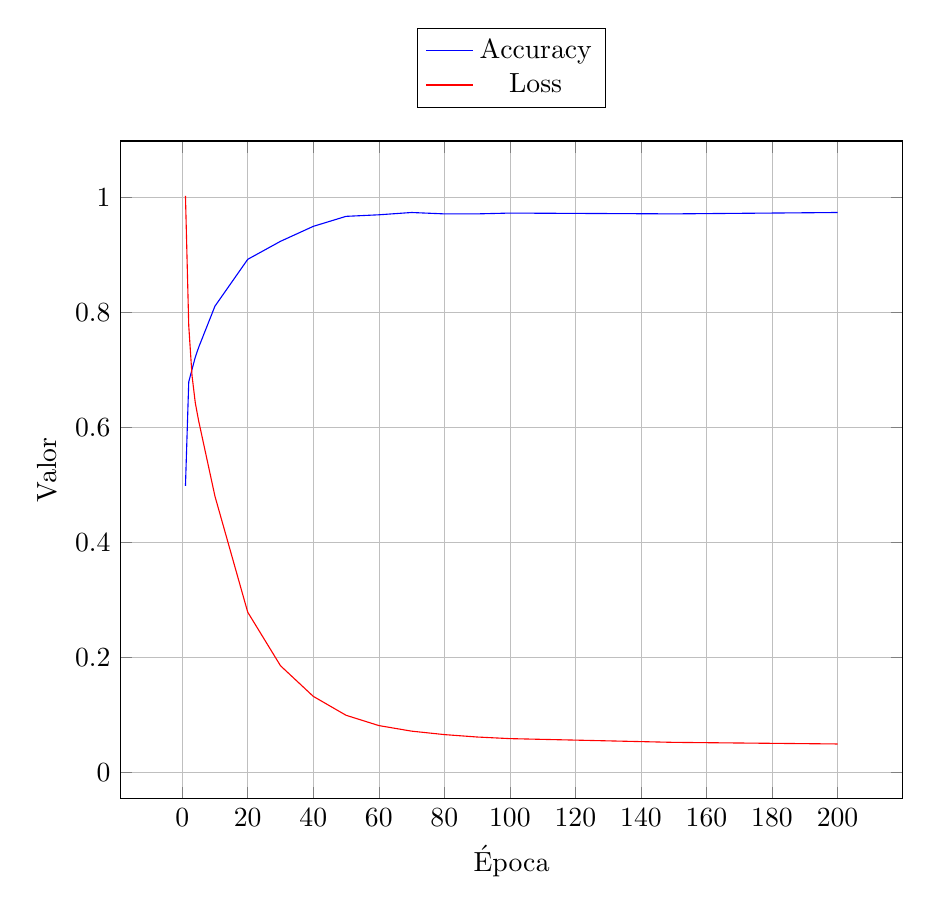
\begin{tikzpicture}
\begin{axis}[
    width=0.95\linewidth,
    xlabel={Época},
    ylabel={Valor},
    legend style={at={(0.5,1.05)}, anchor=south},
    grid=both,
    grid style={line width=.1pt, draw=gray!30},
    major grid style={line width=.2pt,draw=gray!50},
]
\addplot[color=blue]
table[row sep=crcr]{
epoch accuracy\\
1 0.4985\\
2 0.6792\\
3 0.7009\\
4 0.7222\\
5 0.7389\\
10 0.8109\\
20 0.8923\\
30 0.9236\\
40 0.9496\\
50 0.9670\\
60 0.9697\\
70 0.9737\\
80 0.9713\\
90 0.9713\\
100 0.9727\\
150 0.9713\\
200 0.9737\\
};

\addplot[color=red]
table[row sep=crcr]{
epoch loss\\
1 1.0027\\
2 0.7772\\
3 0.6903\\
4 0.6429\\
5 0.6122\\
10 0.4805\\
20 0.2790\\
30 0.1859\\
40 0.1327\\
50 0.0998\\
60 0.0819\\
70 0.0722\\
80 0.0662\\
90 0.0620\\
100 0.0592\\
150 0.0527\\
200 0.0499\\
};



\legend{Accuracy, Loss}

\end{axis}
\end{tikzpicture}
\caption{Evolución de la \textit{accuracy} y la \textit{loss} durante el entrenamiento.}
\label{fig:training_plot_pgf}
\end{figure}

\vspace{9em}


Se puede observar que a partir de unas 30 épocas el crecimiento de la precisión es escaso, y que a partir de unas 50 épocas, la precision del algoritmo, se mantiene estable. Si se miran los datos en detalle, se podría ver que en algunos puntos empeora unas milesimas, pero de nuevo las gana en los siguientes. Por otro lado, si se puede ver como baja la perdida sin quedarse tan estancada, aunque posiblemente acabará de nuevo en una asíntota.


\begin{table}[h]
\centering
\caption{Rendimiento del modelo en función del número de partidas utilizadas}
\label{tab:partidas_accuracy_loss}
\begin{tabular}{c c c c}
\hline
\textbf{Partidas (p)} & \textbf{Accuracy (A)} & \textbf{Loss (L)} & \textbf{Ejemplos (e)} \\
\hline
50  & 0.8019 & 0.4805 & 2999 \\
100 & 0.8273 & 0.4261 & 5998 \\
25  & 0.8532 & 0.3894 & 1499 \\
10  & 0.9332 & 0.2142 & 599  \\
5   & 0.9867 & 0.1275 & 300  \\
1   & 0.9167 & 0.4261 & 60   \\
\hline
\end{tabular}
\end{table}


Se puede observar con la tabla como el modelo con menos partidas memoriza ciertos patrones sin aprenderlos realmente, subiendo descaradamente la precisión y bajando esta según estos patrones dejan de ser tan completos. Así es como de nuevo crece la precisión con 100 partidas tras haber bajado hasta las 50.



\section{Uso de la inteligencia artificial}\label{sec:Uso de IA}
En este proyecto se han usado herramientas de inteligencia artificial generativa como apoyo. Se han usado Claude, ChatGPT y Copilot para Visual Studio. No obstante, a pesar de haber sido de ayuda ha habido una revisión total de cada cosa que ha generado, pues a veces usaba una nomenclatura distinta o simplemente no lo daba correcto.

Para trasladar a \LaTeX{} como pseudocódigo las funciones que se querían explicar, simplemente se le pasaba el código y se hacía la pregunta..
Se ha preguntado a la IA para hacer las tablas en \LaTeX{}, se le ha pasado la información que se quería mostrar y ha generado correctamente las tablas en formato \LaTeX{}.

Para el tablero con PyGame, a pesar de que como se menciona en el documento hemos reutilizado como base un tablero de un proyecto de otra asignatura le pedimos que nos creara una opción para poder elegir con que color jugar, ya que al principio solo teníamos uno predeterminado que no se podía cambiar desde la propia interfaz. También le pedimos que la IA pudiera jugar contra nosotros de forma que tu colocas tu ficha y la IA juega la suya en su turno. Los resultados fueron muy favorables.

Para el entrenamiento se le pidió a la IA que configurase el entorno, ya que con ciertas versiones de Python no soportaban Keras. También pedimos una primera versión para poder tener una idea de que se nos pedía exactamente, pues al principio no estaba muy claro claro.

Para el juego en sí se le pidió a la IA una idea general de como llevar a cabo el desarrollo del tablero, pues estaba clara cual sería la mejor manera de implementarlo y buscar y aplicar los movimientos.

Para el algoritmo UCT se le pidió ayuda para pasar la función \textit{Best\_child} de pseudocódigo a código pues nos daba fallo inicialmente. También para \textit{Default\_policy} porque nuestra primera implementación tenía algunos bugs. También para ahorrar tiempo le pedíamos a la IA que nos pasara a código las expresiones matemáticas que salían, como las diversas raíces cuadradas que hay que implementar.

Se han añadido algunos comentarios al código por medio de la ia para hacerlo más comprensible.




\section{Conclusiones}\label{sec:Conclusiones}
En este trabajo se ha desarrollado una inteligencia artificial capaz de jugar a Otelo mediante la combinación de Monte Carlo Tree Search con el algoritmo UCT y una red neuronal entrenada a partir de partidas generadas por self-play. Además de implementar el juego y una interfaz gráfica para la interacción con el usuario, se llevaron a cabo diversos experimentos para evaluar el impacto de distintos criterios de selección y parámetros de entrenamiento.
Además se puede jugar correctamente una partida de Otelo contra la máquina en una interfaz gráfica, usando los modelos que se han generado.

Con esos modelos entrenados se han hecho varios experimentos para comprobar la influencia de los criterios de selección del algoritmo UCT y de los principales parámetros de entrenamiento de la red neuronal. Los resultados muestran que el uso de una red neuronal como función de evaluación mejora la eficiencia del proceso de búsqueda y que los criterios \textit{max-robust} y \textit{secure} obtienen, en general, los mejores resultados. 

Asimismo, se comprobó la influencia de las épocas en los entrenamientos según los criterios de decisión. Se observa que se necesitan al menos 30 para tener unos datos de precisión y pérdida significativos, mientras que incrementar el número de épocas no merece la pena pues la diferencia resultados es muy marginal. En conclusión, el trabajo demuestra la viabilidad de combinar UCT y redes neuronales para construir un agente inteligente de Otelo capaz de aprender mediante self-play.

Como resultados de los experimentos hechos con los cambios en los datos de learning rate, batch size, épocas y partidas, cogiendo los datos más óptimos de cada uno (5 partidas, 50 épocas, 1 batch size y 0,01 de learning rate) nos da una precisión máxima de 0,9967 en la época 39, con una perdida de 0,0235. 

Como trabajo futuro se podrían hacer entrenamientos de números aún más grandes de partidas, pues se ha llegado a 100 solo porque tardaban demasiado los entrenamientos. Debido a esto se podría también explorar la posibilidad bajar el tiempo de entrenamiento del modelo.
Adicionalmente se podrían implementar otros tipos de redes neuronales, como una red convolucional, para analizar las diferencias de resultados y poder saber si otra red es más efectiva.

\begin{thebibliography}{00}
\bibitem{b1} S. Russell and P. Norvig, Artificial Intelligence: A Modern Approach, 4th ed., Pearson,
2020, ch. 5, “Adversarial Search”.
\bibitem{b2}  C. B. Browne, E. Powley, D. Whitehouse, S. M. Lucas, P. I. Cowling, P. Rohlfshagen, S. Ta
vener, D. Perez, S. Samothrakis, and S. Colton, “A Survey of Monte Carlo Tree Search
Methods,”IEEE Transactions on Computational Intelligence and AI in Games,vol.4,no.1,
pp. 1–43, 2012, doi: 10.1109/TCIAIG.2012.2186810.
\bibitem{b3} Los primeros programas de IA capaces de aprender
Inteligencia Artificial, Profundizando en el Big Data, BigData UMA

\bibitem{b4} Aprendiendo a jugar a Otelo
Propuesta de trabajo para la asignatura Inteligencia Artificial
Profesor: Ignacio Pérez Hurtado de Mendoza
Grado en Ingeniería Informática- Ingeniería del Software
Curso 2025/2026

\end{thebibliography}


\end{document}
